\chapter{Literature review}\label{chapter:warmup}

The following chapter provides an overview of the past research related to the warm-up as a preparatory exercise prior performing physical activity and conceptually related works in the domain of gamified solutions relevant to fitness and exercise. To impose structure, first the basic concepts related to warm-up and an overview of studies and results regarding the benefits of warm-up is given. Following, the concept of gamification is introduced and most relevant ... in ... At the end of this chapter, a comparison between the presented approaches and our solution is made.
\section{Warm up in sports}
\subsection{Introduction}
Despite very contrasting believes and limited scientific evidence regarding it's effectiveness in many situations, warm-up (WU) has become a standard practice among professional and
recreational athletes \cite{bishop2003warm1, bishop2003warm2, shellock1985warming}. WU in sports is defined as a period of preparatory exercise which is carried out in order to prepare the athlete for the demands of the subsequent physical activity \cite{karvonen1992importance, woods2007warm, hedrick1992exercise}.
%karvonen skini i procitaj
Typically, WU includes a short and low-intensity preparatory activity which is followed by a stretching routine and sport specific exercise \cite{safran1989warm}. 
The purpose of WU is to enhance the subsequent competition or training performance and improve muscle dynamics to reduce the risk of sport-related injury\cite{bishop2003warm1, shellock1985warming, knudson2008warm}. 
 %HERE MENTION THE STUDIES THAT SAY THIS DOESNT HELP.  CHECK LEMON ILIEV
Nonetheless, there is still deficiency of scientific evidence on what kind of WU can influence both muscle damage prevention and performance improvement \cite{safran1989warm}.\\ %cite
\subsection{WU benefits}
Fradkin \textit{et al.} carried out a systematic review and meta-analysis of relevant studies concerning the benefits of WU on the performance. They found that an adequate WU supports an improvement in performance in 79\% of the research studies analyzed. Furthermore, they pointed out that there exist little evidence supporting detrimental effects WU might have on performance and sports participants.
WU can affect the performance via variety of temperature and non-temperature related mechanisms \cite{bishop2003warm1}. 
%By performing a low intensity training routine before taking part in more demanding exercise, an increase in one's body temperature \(Magnusson 
%et al., 2000\) and muscle blood flow occurs \(Tiidus \& Shoemaker, 1995\).  
The most relevant effects of WU can be attributed to physiological mechanisms like increased muscle temperature, decreased resistance of muscle and joints (decreased stiffness), increased oxygen delivery to muscles, increased nerve-conduction rate and speeding of metabolic reactions \cite{bishop2003warm1}. 
However, the benefits of WU are not exclusively physical. Apart from the physiological changes a body undergoes during this preparatory period, it has been hypothesized that a possible psychological benefit can also be gained by following a proper WU routine \cite{bishop2003warm1,shellock1985warming}.
It has been suggested that WU can serve as preparatory phase providing time for athlete to concentrate and mentally prepare for the forthcoming exercise \cite{shellock1985warming}. 
%Thus, possible psychological benefits is increased mental preparedness for the forthcoming exercise\cite{bishop2003warm1}. 
For instance, in the study that investigated the link between a WU and psychological processes, Ladvig (2013) reported that athletes who reported performed a proper WU routine before engaging in more demanding physical activity demonstrated significantly higher levels of exercise related motivation and enjoyment. Thus increased motivation and enjoyment is an additional psychological benefit of WU \cite{ladwig2013psychological}.
 %findings of this theisis: http://aut.researchgateway.ac.nz/bitstream/handle/10292/325/WeerapongP.pdf?sequence=1
\\Apart from physiological and psychological benefits, WU has been suggested to have an important role in sports-related injury prevention \cite{shellock1985warming}. Unfortunatelly, there exist no high-quality research studies in order to draw definite conclusion as to the effect WU has on sports-related injury prevention \cite{fields2007should}. Safran, \textit{et al.} proposed a possible bio-mechanical explanation for injury reduction with WU. The results of this study reported that warmed-up muscles in the animal models can elongate more before failure caused by increased force and length of stretch \cite{safran1989warm}. In the study of Fradkin, \textit{et al.} the current evidence regarding WU in injury prevention has been assessed. Out of five high-quality studies with sufficient data that have been systematically reviewed, three studies reported significant injury related reduction by performing WU before the physical activity while in other two no benefits were reported. Overall, based on the weight of evidence, it has been concluded in favor of WU to decrease the risk of injury.\\
%Furthermore, Nosaka and Clarckson found that high and low intensities of WU could reduce the magnitude musculatory damage ... They proposed that 
%A search of the literature identified only one published research paper on the effects of warm-up on the severity of muscle damage (Nosaka & Clarkson, 1997).  Nosaka and Clarkson (1997) found that both high (100 repetitions of maximal concentric contraction) and low (100 repetitions of minimal concentric contraction) intensities of 
%warm-up could reduce the magnitude of mu
%scle damage as indicated by reduced 
%soreness sensation, strength and range of 
%motion loss, swelling, and creatine kinase 
%activity.  The authors proposed that warm-up 
%might help to increase muscle temperature 
%and circulation, and consequen
%tly, increase muscle and conne
%ctive tissue el
%asticity
%the majority of effects of warm up have been attributed to temperature related mechanism
\subsection{WU types}
There exist various types of WU procedures professional and recreational athletes use as a preparatory phase for the physically more demanding exercise preparation. It is important to distinguish between WU and stretching activities. While WU mainly focuses on core body temperature elevation, stretching involves movements that stretch the muscle in order to increase the range of motions of joints or group of joints \cite{knudson2008warm}. 
Generally, WU procedures can be classified into active and passive WU procedures, and are centered on increase in core and muscle temperature. However, active and passive WU accomplish this objective through different approaches. The former involves raising muscle or core temperature by some external means (e.g. hot showers, saunas), while the latter aims to increase the body temperature through active movements of the major muscle groups (e.g. jogging, cycling, swimming) \cite{shellock1985warming, bishop2003warm2}. The most effective WU that could potentially effect the subsequent performance generally depends on the duration, intensity and the nature of the sports activity to be performed \cite{bishop2003warm2}. As each sport has its own unique requirements, it is difficult to specify a general WU routine that is beneficial and have positive impact by maximizing the subsequent performance. Nonetheless, it is suggested that a proper WU should use general, whole-body movements and last 5-10 minutes which is followed by a 5 minutes recovery period \cite{bishop2003warm2}.  
%dodaj za fatigue
%Several studies were conducted in the 1950s-1970s to investigate the effects of warming-up on athletic performance
%(Richards, 1968). In this context, approximately 60% of these studies found that warm-up was better
%to perform than no warm-up, whereas ~11% found that no warm-up was better, and the remaining ~29% found
%no significant differences between different protocols of warm-up and no warm-up (Blank, 1955). 
%tu sad das ove linkove
%(Generally, a warm-up to minimize impairments and enhance performance should be composed of a submaximal intensity aerobic activity followed by large amplitude dynamic stretching and then completed with sport-specific dynamic activities.
%these say that some stretching is ok
%http://www.jospt.org/doi/pdf/10.2519/jospt.1994.19.1.12
%https://www.ncbi.nlm.nih.gov/pubmed/21373870
%The efficacy, and characteristics, of warm-up and re-warm-up practices in soccer players: a systematic review. This review demonstrated that a static stretching WU reduced acute subsequent performance, while WU activities that include dynamic stretching, PAP-based exercises, and the FIFA 11+ can elicit positive effects in soccer players. The efficacy of an active RWU during half-time is also justified.
%ovo se placa nesto 
 %http://greatist.com/fitness/stretching-dynamic-warmup-040413
\\Although, considering the aforementioned benefits, is widely recommended to undertake the practice of WU, many amateur and recreational athletes do not seem to perform a proper WU before an exercise \cite{fradkin2010effects}. The reasons for this are manifold. Some people do not realize the importance of WU, find it tiresome or pressed for time and eager for instantaneous results, start with the more strenuous activity immediately. A recent survey carried out by Fradkin, \textit{et al.} including 1040 golfers and their WU habits, revealed the most common reasons for not warming-up. The survey showed that out of all the questioned golfers, over 70\% never or rarely warm-up. The most common reasons for not performing a proper WU routine were the perception that WU is needless (38.7\%), lack of time (36.4\%) and that they do not want to be bothered with this routine (33.7\%).
% A survey of 1040 randomly selected golfers was conducted over a 3-week period in July 1999. Information about golf participation, usual warm-up habits and reasons for these warm-up behaviours was obtained by a verbally administered self-report survey. Over 70% of the surveyed golfers stated that they never or seldom warm-up, with only 3.8% reporting warming-up on every occasion. The most common reasons why golfers warmed-up included to play better (74.5%), to prevent injury (27.0%), and because everyone else does (13.2%). Common reasons for not warming-up were the perception that they don't need to (38.7%), don't have enough time (36.4%) and can't be bothered (33.7%).
These results suggest that educational and motivational solutions with primary focus on benefits of WU, including injury prevention, need to be developed and implemented in order to increase the proportion of athletes who engage in WU routines before every strenuous exercise. One possible solution is the usage of \textit{gamification} in motivating athletes to perform WU more regularly. 
\pagebreak
\section{Gamification}
\subsection{Definition}
%http://link.springer.com/chapter/10.1007%2F978-3-319-07127-5_23
%(http://www.enterprise-gamification.com/mediawiki/index.php?title=Category:Gamification_Design_Elements)
% are commonly used 
%check this here https://badgeville.com/wiki/health
%% add gamification example reference
% http://www.enterprise-gamification.com/mediawiki/index.php?title=Gamification_Examples
In recent years, there have been an tremendous increase in popularity of video games inspired software solutions designed to address issues in variety of functional areas, incentivize consumer behavior or increase motivation and desire for achievement. What these software solutions all have in common is that they are based on the concept of \textit{gamification}. This term has begun to rise in popularity in 2010 (Figure \ref{fig:buzz}), and since then has been a trending topic. %ovde dodaj 
%It has proved to be an effective tool for certain businesses for developing new skills, solve problems, improve results or address.
\begin{figure}[h]
    \centering
    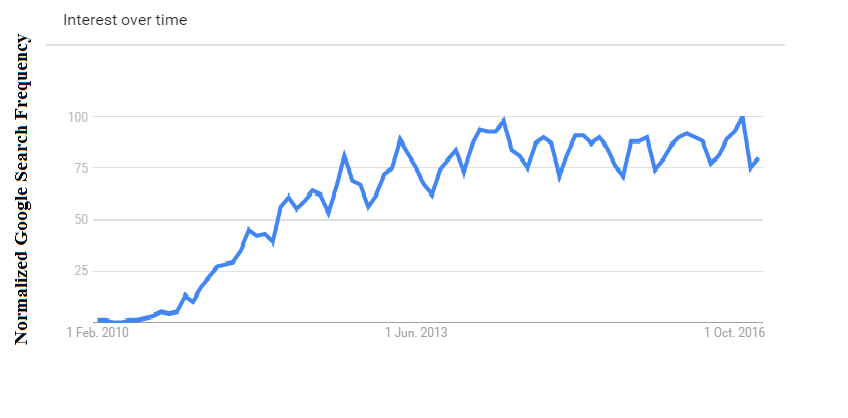
\includegraphics[width=\textwidth]{buzz}
    \caption{Google search frequency of the term \textit{gamification} from Janauary 2010 through January 2017. Data source: Google Trends, www.google.com/trends}
    \label{fig:buzz}
\end{figure}
Gamification is being used and studied in various domains, from education and academic performance to health care, finance, company culture building and recruitment, to name a few \cite{gamificationExamples, gamificationWiki, enterpriseGamify}. Large companies like Nike \cite{nikePlus}, Deloitte \cite{deloitte}, Starbucks \cite{starbucks}, Coca Cola \cite{coke} and Toyota \cite{toyota} have all used gamified solutions. %cite the examples and change this sentance. cite https://badgeville.com/wiki/Gamification_Examples
Moreover, there is an increasing number of startups that base their services on the gamification concept \cite{codeacademy} or offer assistance to enterprises to gamify their existing services \cite{badgeville}. Hamari \textit{et al.} reported on an increasing popularity of gamification related researches in the academia \cite{hamari2014does}. Figure \ref{fig:pub} gives an overview of the increase of writing on this topic. The figure includes only the number of publications for every year for the term \textit{gamification} and excludes patents and citations. 
\begin{figure}[h]
    \centering
    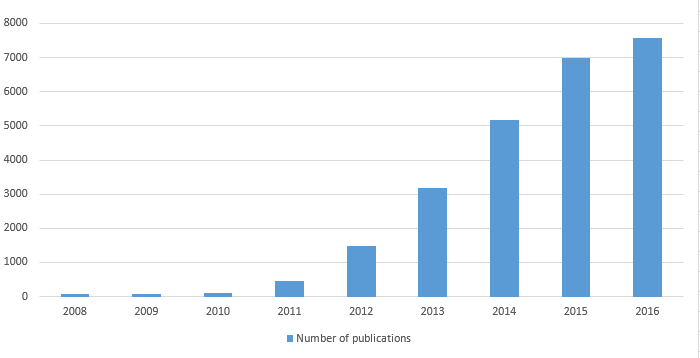
\includegraphics[width=\textwidth]{pub}
    \caption{Search hits on 'gamification'. Data source: www.scholar.google.com}
    \label{fig:pub}
\end{figure}
It is worth noticing that the appearance of term gamification publication titles' has been increasing more rapidly than search hits for the same term (see Figure \ref{fig:buzz}). This suggests that gamification is becoming more popular in academic inquiry. 
Detering \textit{et al.} (2011) define gamification as ``the use of game design elements in a non-game context''  \cite{deterding2011game}. In parallel with this term, a verb \textit{to gamify} has been defined. It's meaning reffers to applying game mechanics to supercharge user engagement, loyalty and fun \cite{toGamify}. It should be noted that the definition of gamification outlined by Detering \textit{et al.} relates to \textit{games} and not \textit{play} \cite{deterding2011game}. Even though often used interchangeably, there exists a complex relationship between these two concept and clear distinction can be made. That is, according to the forms they take in the world, \textit{play} can be interpreted as a broader category that includes \textit{game} as a subset \cite{salen2004rules}. Play is normally assumed to be a free-form activity lacking constraints engaged in for pleasure and amusement rather than a serious or practical purpose, whereas games provide context for actions and are limited in action by fixed rules \cite{juul2011half}. In addition, Salen and Zimmerman define game as a system where players engage in an artificial conflict which is defined by rules that limit players behavior and define the game, that can result in a quantifiable outcome or goal \cite{salen2004rules}.
Game design elements represent parts of games used as a building block for creating gamified applications. They are tools and rules that define the overall context of game \cite{gamDesElem}. This means that the definition distinguishes gamification from other systems that employ full-fledged games rather than elements of game design only. Furthermore, it does not include all game elements either, only a subcategory called game design elements. %ova dve poslednje recenice odavde, izmeni 
%http://ludus.hu/en/gamification/
Game design elements are themselves difficult to specify and often are described on varying levels of abstraction. Derived from the available literature, Deterding et al. found that previously identified game elements fell into five distinct levels of abstraction. Table \ref{table:gameElements} lists the five levels of game elements, ordered from concrete to abstract.

\pagebreak
% Please add the following required packages to your document preamble:
% \usepackage[normalem]{ulem}
% \useunder{\uline}{\ul}{}
\begin{table}[]
\centering
\caption{Taxonomy of game design elements by level of abstraction}
\label{table:gameElements}
\begin{tabular}{lll}
\hline
\textbf{Level} & \textbf{Description} & \textbf{Example} \\ \hline
\begin{tabular}[c]{@{}l@{}}Game interface\\ design patterns\end{tabular} & \begin{tabular}[c]{@{}l@{}}Common, successful interaction\\  design components and design \\ solutions for a known problem\\  in a context, including prototypical\\  implementations\end{tabular} & \begin{tabular}[c]{@{}l@{}}Badge, leaderboard, \\ level\end{tabular} \\ \hline
\begin{tabular}[c]{@{}l@{}}Game design\\ patterns and\\ mechanics\end{tabular} & \begin{tabular}[c]{@{}l@{}}Commonly reoccurring parts of \\ the design of a game that\\  concern gameplay\end{tabular} & \begin{tabular}[c]{@{}l@{}}Time constraint, \\ limited resources, turns\end{tabular} \\ \hline
\begin{tabular}[c]{@{}l@{}}Game design\\ principles and\\ heuristics\end{tabular} & \begin{tabular}[c]{@{}l@{}}Evaluative guidelines to approach a\\  design problem or analyze a given\\ design solution\end{tabular} & \begin{tabular}[c]{@{}l@{}}Enduring play,\\ clear goals, \\ variety of game styles\end{tabular} \\ \hline
Game models & \begin{tabular}[c]{@{}l@{}}Conceptual models of the components of\\  games or game experience\end{tabular} & \begin{tabular}[c]{@{}l@{}}
MDA; challenge, \\ fantasy, curiosity;\\ game design atoms; \\ Core Elements of the \\ Gaming Experience \end{tabular} \\ \hline
\begin{tabular}[c]{@{}l@{}}Game design\\ methods\end{tabular} & \begin{tabular}[c]{@{}l@{}}Game design-specific\\  practices and processes\end{tabular} & \begin{tabular}[c]{@{}l@{}}Playtesting,\\ playcentric design, \\ value conscious\\ game design\end{tabular} \\ \hline
\end{tabular}
\end{table}

%With respect to the use of game design elements, gamification studies classified gamification elements differently \cite{schobel2016agony}.% Sch{\"o}bel \textit{et al.} carried out a literature review to analyze the gamification elements used in various research studies.
%prezentacija o game vs play http://gamification-research.org/2012/04/defining-gamification/
%detering definise elements of game design. five leveles.
Lastly, a non-game context refers to applications which main purpose is beyond pure entertainment. Some examples of contexts where gamification has been successfully applied include: business, personal improvement, education, health and fitness. %ovo dopuni
The definition of gamification is closely related to similar pre-existing concepts such as serious games and playful interaction \cite{deterding2011game}. However, the concept of gamification can be differentiated from these similar phenomena on a two-by-two matrix introduced by Detering \textit{et al.} (Figure \ref{fig:mesh1}). 

\begin{figure}[h]
    \centering
    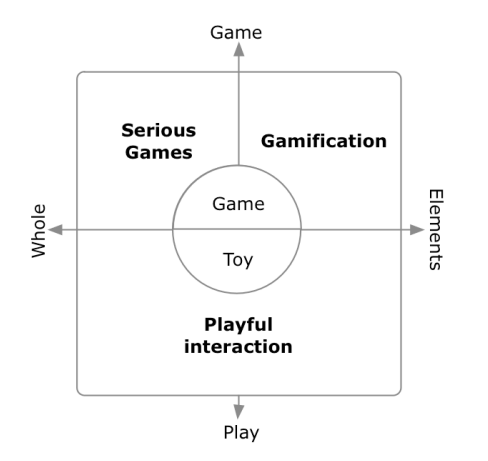
\includegraphics[width=0.50\textwidth]{gamification-btw-game-and-play2}
    \caption{The matrix distinguishing the concepts related to gamification}
    \label{fig:mesh1}
\end{figure}
In figure \ref{fig:mesh1}, along one axis Detering \textit{et al.} a distinction between gaming and playing is made, and on the other between whole or partial artefacts. They place gamification or gameful design in the quadrant involving games and partial artefacts, meaning that gamification uses gameful design rather than playful design and game elements rather than full-fledged games. 
 
 
%% add gamification example reference
% 

In theory, any context, task or process can be gamified \cite{muntean2011raising}. %skini i procitaj Muntean!! 

The main goal of gamification is to engage the users 
Gamification’s main goal is to rise the engagement of users by using game-like techniques such as
scoreboards and personalized fast feedback (Flatla et al, 2011) making people feel more ownership
and purpose when engaging with tasks (Pavlus, 2010). 
\cite{burke2016gamify}

Figure 1: 
Gamification in Health and Fitness has rapidly emerged over the past decade as a tool to promote health and wellness. It is a broad term referring to the use of game thinking and game mechanics in a non-game context to engage users and solve problems. The concept is used to incentivise users to achieve their goals and increase user engagement. The best examples of gamification are in the Health and Fitness industry, where games encourage exercise by turning physical activity into a game and by delivering health interventions for bad habits cessation, like smoking, overeating or poor hydration, and medication adherence. Application of mobile and wearable devices have proven to be effective platforms for health and fitness games due to its wide adaptation, ease of use and continuous proximity to the users and patients.
Since gamification can be applied to almost any business model, serious or not,
for this thesis, we restrict our concern of gamification to the solving of serious issues. In
particular, we are focused on gamification of education and behavior change related to the
serious world issue of childhood obesity
